\documentclass[25pt, a0paper,
margin=0mm, innermargin=15mm, blockverticalspace=5mm, colspace=15mm, subcolspace=1mm]{tikzposter}
\usepackage{trace}
\usepackage{amsmath}
\usepackage{booktabs}
\usepackage{multirow}
\usepackage{multicol}
\usepackage{mathtools}
\usepackage{cmbright}
\usepackage[backend=biber]{biblatex}
\addbibresource{biblio.bib}
\usepackage{fontspec}
\usepackage{bm}
\newfontfeature{Microtype}{protrusion=default;expansion=default;}
\tikzposterlatexaffectionproofoff

\DeclareMathOperator\logit{logit}
\DeclareMathOperator\probit{probit}
\def\R{\mathbf{R}}
\def\N{\mathcal{N}}
\def\pij{p_{ij}}
\def\logitp{\logit{} p_{ij}}

\usepackage{graphicx}
\usepackage{wrapfig}
\usepackage{hyperref}
\usepackage{xcolor}
\hypersetup{
    colorlinks,
    citecolor={blue!80!black},
}
\newcommand{\email}[1]{\href{mailto:#1}{\textsf{#1}}}
\title{\parbox{\linewidth}{\begin{center}\textbf{Deep Factorization Machines for Knowledge Tracing}\end{center}}}
\author{\centering
  \begin{tabular}{cc}
    \textbf{Jill-Jênn Vie} \\
    RIKEN Center for Advanced Intelligence Project (AIP)\\
Tokyo, Japan\\
\texttt{vie@jill-jenn.net}
  \end{tabular}
    }

\usetheme{Simple}

\usecolorpalette{BrownBlueOrange}
\makeatletter
\renewcommand\TP@maketitle{
   \begin{minipage}{0.98\linewidth}
        \centering
        \color{titlefgcolor}
        {\bfseries \Huge \sc \@title \par}
        \vspace*{1em}
        {\Large
          \@author \par}
    \end{minipage}
}
\makeatother

\usepackage{theorem}
\theoremstyle{myplain}
\newtheorem{transformation}{Transformation}
\newcommand{\concprio}{\rangle\kern-0.15em\rangle}

\usepackage{tikz-qtree}

\usetikzlibrary{arrows,arrows.meta,automata,shapes,intersections,mindmap,trees,shadows,fit,positioning,calc,matrix,decorations,chains,external,3d}
\makeatletter
\tikzoption{canvas is xy plane at z}[]{%
\def\tikz@plane@origin{\pgfpointxyz{0}{0}{#1}}%
\def\tikz@plane@x{\pgfpointxyz{1}{0}{#1}}%
\def\tikz@plane@y{\pgfpointxyz{0}{1}{#1}}%
\tikz@canvas@is@plane
}
\makeatother
\usepackage{listings}
\usepackage{enumitem}
\usepackage{booktabs}
\newcommand{\Gproc}{\textbf{proc }}
\newcommand{\GendProc}{\textbf{ endProc}}
\newcommand{\Gif}{\textbf{if }}
\newcommand{\Gthen}{\textbf{ then }}
\newcommand{\Gelse}{\textbf{ else }}
\newcommand{\Gwhile}{\textbf{while }}
\newcommand{\Gdo}{\textbf{ do }}
\newcommand{\mprefer}{\,\rangle\,}
\newcommand{\GendIf}{\textbf{ endIf }}
\newcommand{\GendWhile}{\textbf{ endWhile }}
\newcommand{\affp}{\textit{aff\/}_p}
\newcommand{\set}[1]{\{#1\}}

\newcommand{\Gleft}[1]{G_{#1}^{\textit{left}}}
\newcommand{\Gright}[1]{G_{#1}^{\textit{right}}}
\newcommand{\Gmiddle}[1]{G_{#1}}

\newcommand{\prefer}{\rangle}

\newcommand{\alert}[1]{{\color{red!70!black} #1}}

\newcommand{\bs}{\textbackslash}   % backslash
\newcommand{\cmd}[1]{{\bf \color{red}#1}}   % highlights command

\graphicspath{{./}{../images/}}

\usenotestyle{Sticky}

\usepackage{mdframed}
\newmdenv[topline=false,bottomline=false,rightline=false,skipabove=0pt,skipbelow=0pt,innertopmargin=0pt,innerbottommargin=0pt]{sidebox}
\def\HyperFirstAtBeginDocument#1{#1}  % lolwut https://tex.stackexchange.com/a/309895/7144

\begin{document}
\maketitle[width=\linewidth,titletotopverticalspace=0pt]

% Here it starts

\definecolor{pixblue}{RGB}{53,81,250}
\colorlet{innerblocktitlebgcolor}{pixblue}

\begin{columns} % Blocks will be placed into columns
    
    \column{.48}
    \block[roundedcorners=40]{Problem: Knowledge Tracing for Language Learning}{
        We want to \alert{predict the correctness} of students over words.\\
        Each student can attempt to write a certain word multiple times, and learns in-between.\\
        \textbf{Fit:} Ordered triplets $(i, j, o) \in I \times J \times \{0, 1\}$\\
        $\Rightarrow$ Student $i$ attempted word $j$ and wrote it correctly/incorrectly.\\
        \textbf{Predict:} $(i, j, ?)$ for new triplets.
    }
    \block[roundedcorners=40]{Existing Models}{
        \begin{itemize}
            \item \textbf{Prediction of sequences}: Bayesian Knowledge Tracing (BKT $:=$ HMM)\\ Deep Knowledge Tracing (DKT $:=$ LSTM) \autocite{piech2015deep}
            \item \textbf{Factor Analysis}: Item Response Theory (IRT), Performance Factor Analysis (PFA)

            \[ \textnormal{BKT} < \textnormal{PFA} \simeq^{\textnormal{\autocite{xiong2016going}}} \textnormal{DKT} \leq^{\textnormal{\cite{wilson2016back}}} \textnormal{IRT } \alert{\leq^{\textnormal{[this poster]}} \textnormal{KTM}} \]

        \end{itemize}

        \vspace{1cm}
        \innerblock[]{Item Response Theory}{
            Students $i \in I$ have unknown level \alert{$\theta_i$}\\
            Questions $j \in J$ have unknown difficulty \alert{$d_j$}
            \[ \logit p_{ij} = \logit \Pr(\textsf{Student } i \textnormal{ answers correctly } \textsf{question } j) = \alert{\theta_i} - \alert{d_j} \]

            \hfill $\Rightarrow$ \textnormal{ \textbf{really simple, ignores skills \& multiple attempts}}
        }
        Multidimensional counterpart (MIRT): $\logit{} p_{ij}= \langle \bm{\theta_i}, \bm{d_j} \rangle + \delta_j$
        \vspace{1cm}
        \innerblock[]{Performance factor analysis}{
            Students $i \in I$ have unknown level \alert{$\theta_i$}, $W_{ik}$ prior wins and $F_{ik}$ fails over skill $k$\\
            Questions $j \in J$ have requirements $\textnormal{KC}(j) \subseteq K$\\
            Skills $k \in K$ have bias \alert{$\beta_k$} and opportunities to be learned after win \alert{$\gamma_k$} and fail \alert{$\delta_k$}

            \[ \logit{} p_{ij}= \alert{\theta_i} + \sum_{k \in \textnormal{KC}(j)} \alert{\beta_k} + \alert{\gamma_k} W_{ik} + \alert{\delta_k} F_{ik} \]

            \hfill $\Rightarrow$ \textnormal{ \textbf{ignores item difficulty}}
        }
        Additive Factor Model (AFM): only consider attempts of student $i$ over skill $k$ ($\gamma_k = \delta_k$)
    }

    \column{.52}
    \block{Our proposal}{
        \innerblock[]{Deep Factorization Machines}{
            All students $i \in I$ and questions $j \in J$ and past performance are encoded into $x$ (entities)\\
            All entities have a bias \alert{$w_k$} and features \alert{$\bm{v_k}$} to model the pairwise relationships between them

            \[ \psi(p(x)) = \mu + \sum_{k = 1}^N \alert{w_k} x_k + \sum_{1 \leq k < l \leq N} x_k x_l \langle \alert{\bm{v_k}}, \alert{\bm{v_l}} \rangle \]

        }
        KTM $:=$ BFM (Bayesian Factorization Machines \cite{freudenthaler2011bayesian}) for classification
        \begin{itemize}
            \item \textbf{KTM} take IRT, MIRT, PFA as special cases
            \item If $\psi = \probit$, $w_k, v_{kf} \sim \N(\mu, 1/\lambda)$, $\mu \sim \N(0, 1)$, $\lambda \sim \Gamma(1, 1)$,\\
            a \textbf{Gibbs sampler} allows to train efficiently KTM \cite{rendle2012factorization}
        \end{itemize}
    }

    \block{Encoding of entities}{
        Unsupervised problem becomes a supervised problem:

        \vspace{5mm}
        \begin{center}
        \begin{tabular}{c @{\hspace{5cm}}c cc c ccc c ccc c ccc c ccc c@{\hspace{5cm}} c}
\toprule
\multirow{2}[3]{*}{Triplet} & &  \multicolumn{2}{c}{Users}  & & \multicolumn{3}{c}{Items} & & \multicolumn{3}{c}{Skills}  & & \multicolumn{3}{c}{Wins}  & &  \multicolumn{3}{c}{Fails} & & \multirow{2}[3]{*}{Outcome} \\
\cmidrule{3-4}
\cmidrule{6-8}
\cmidrule{10-12}
\cmidrule{14-16}
\cmidrule{18-20}
&&  1 & 2 & & Q$_1$ & Q$_2$ & Q$_3$ & & S$_1$ & S$_2$ & S$_3$ & & S$_1$ & S$_2$ & S$_3$ & & S$_1$ & S$_2$ & S$_3$ \\
\midrule
$(2, 2, 1)$ &&  0 &   1 & &  0 &   1 &   0 &&   1 &   1 &   0 &&   0 &   0 &   0 &&   0 &   0 &   0  && 1 \\
$(2, 2, 0)$ &&  0 &   1 & &  0 &   1 &   0 &&   1 &   1 &   0 &&   1 &   1 &   0 &&   0 &   0 &   0  && 0 \\
$(2, 2, 1)$ &&  0 &   1 & &  0 &   1 &   0 &&   1 &   1 &   0 &&   1 &   1 &   0 &&   1 &   1 &   0  && 1 \\
$(2, 3, 0)$ &&  0 &   1 & &  0 &   0 &   1 &&   0 &   1 &   1 &&   0 &   2 &   0 &&   0 &   1 &   0  && 0 \\
$(2, 3, 1)$ &&  0 &   1 & &  0 &   0 &   1 &&   0 &   1 &   1 &&   0 &   2 &   0 &&   0 &   2 &   1  && 1 \\
$(1, 2, 1)$ &&  1 &   0 & &  0 &   1 &   0 &&   1 &   1 &   0 &&   0 &   0 &   0 &&   0 &   0 &   0  && 1 \\
$(1, 1, 0)$ &&  1 &   0 & &  1 &   0 &   0 &&   0 &   0 &   0 &&   0 &   0 &   0 &&   0 &   0 &   0  && 0 \\
\bottomrule
\end{tabular}

        \end{center}
        \vspace{1cm}

        \begin{minipage}{0.6\linewidth}
            Encoding users + items == IRT\\
            Encoding users + skills + attempts == AFM\\
            Encoding users + skills + wins + fails == PFA\bigskip\\

            What is the influence of the data over the model?            
        \end{minipage}
        \begin{minipage}{0.4\linewidth}
            
\includegraphics[width=\linewidth]{figures/aip.png}
        \end{minipage}
    }

\end{columns}
\begin{columns}
\column{.55}
\block{Various, large-scale educational datasets}{

    \begin{tabular}{lrrrrrrr}
\toprule
         Name &  Users &  Items &  Skills &  Skills per item &  Entries &  Sparsity (user-item) &  Attempts per user \\
\midrule
     fraction &    536 &     20 &       8 &            2.800 &    10720 &                  1.000 &              1.000 \\
    timss2003 &    757 &     23 &      13 &            1.652 &    17411 &                  1.000 &              1.000 \\
  assistments &   4217 &  26688 &     123 &            0.796 &   346860 &                  0.003 &              1.014 \\
     berkeley &   1730 &    234 &      29 &            1.000 &   562201 &                  0.731 &              1.901 \\
     castor6e &  58939 &     17 &       2 &            1.471 &  1001963 &                  1.000 &              1.000 \\
\bottomrule
\end{tabular}
\vspace{1cm}\\
    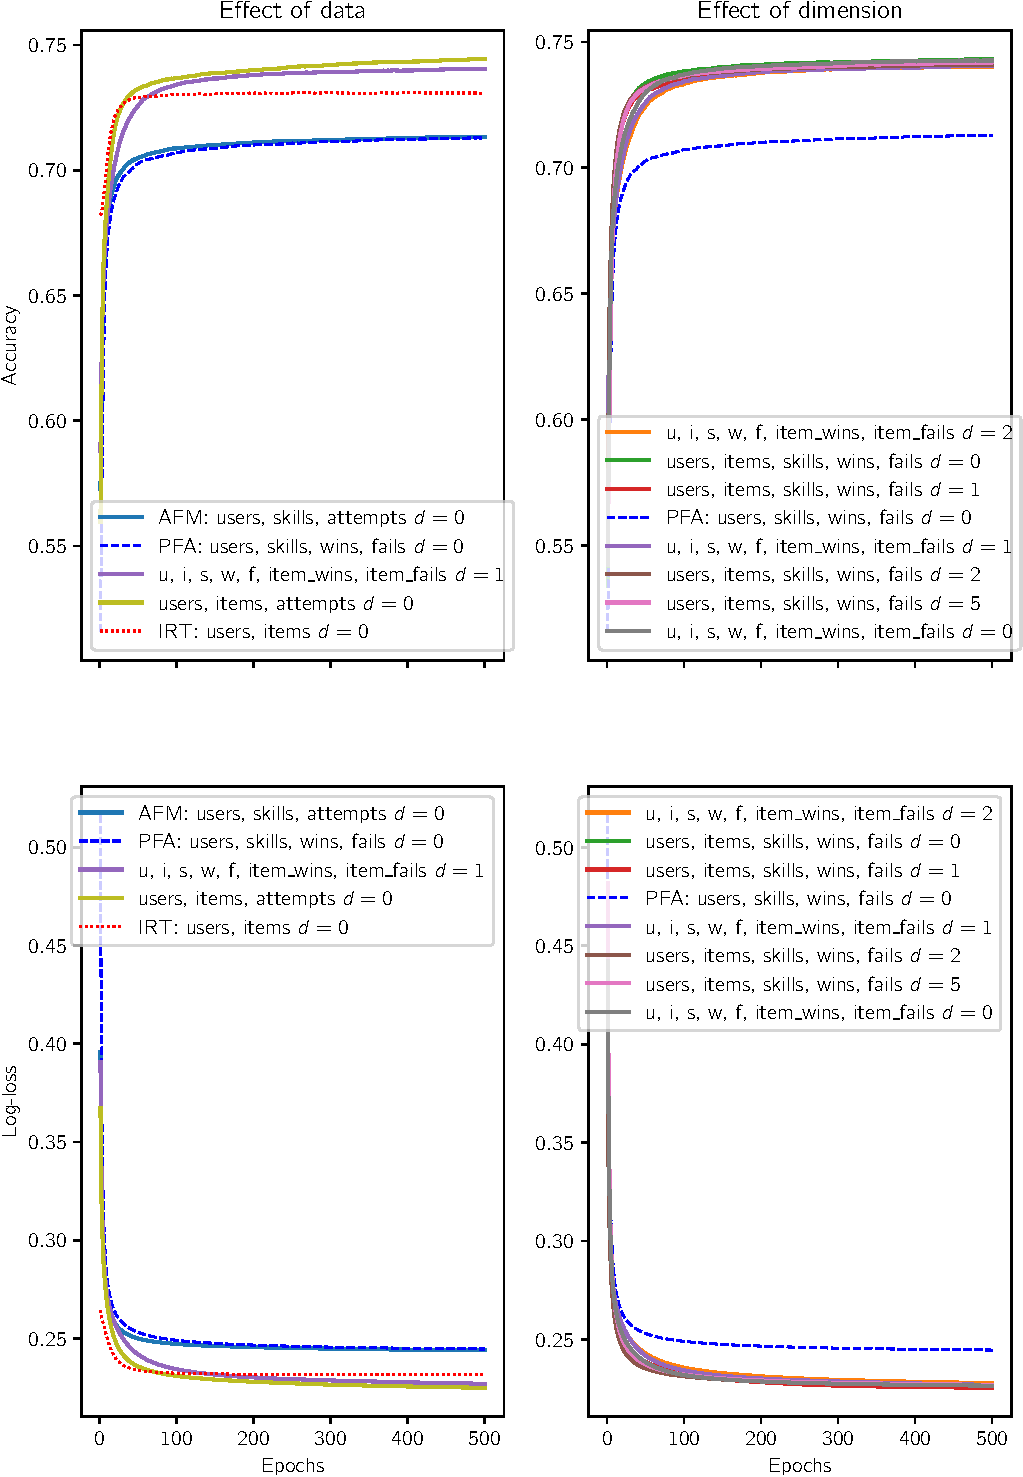
\includegraphics[width=0.50\linewidth]{figures/assistments0-poster.pdf}
    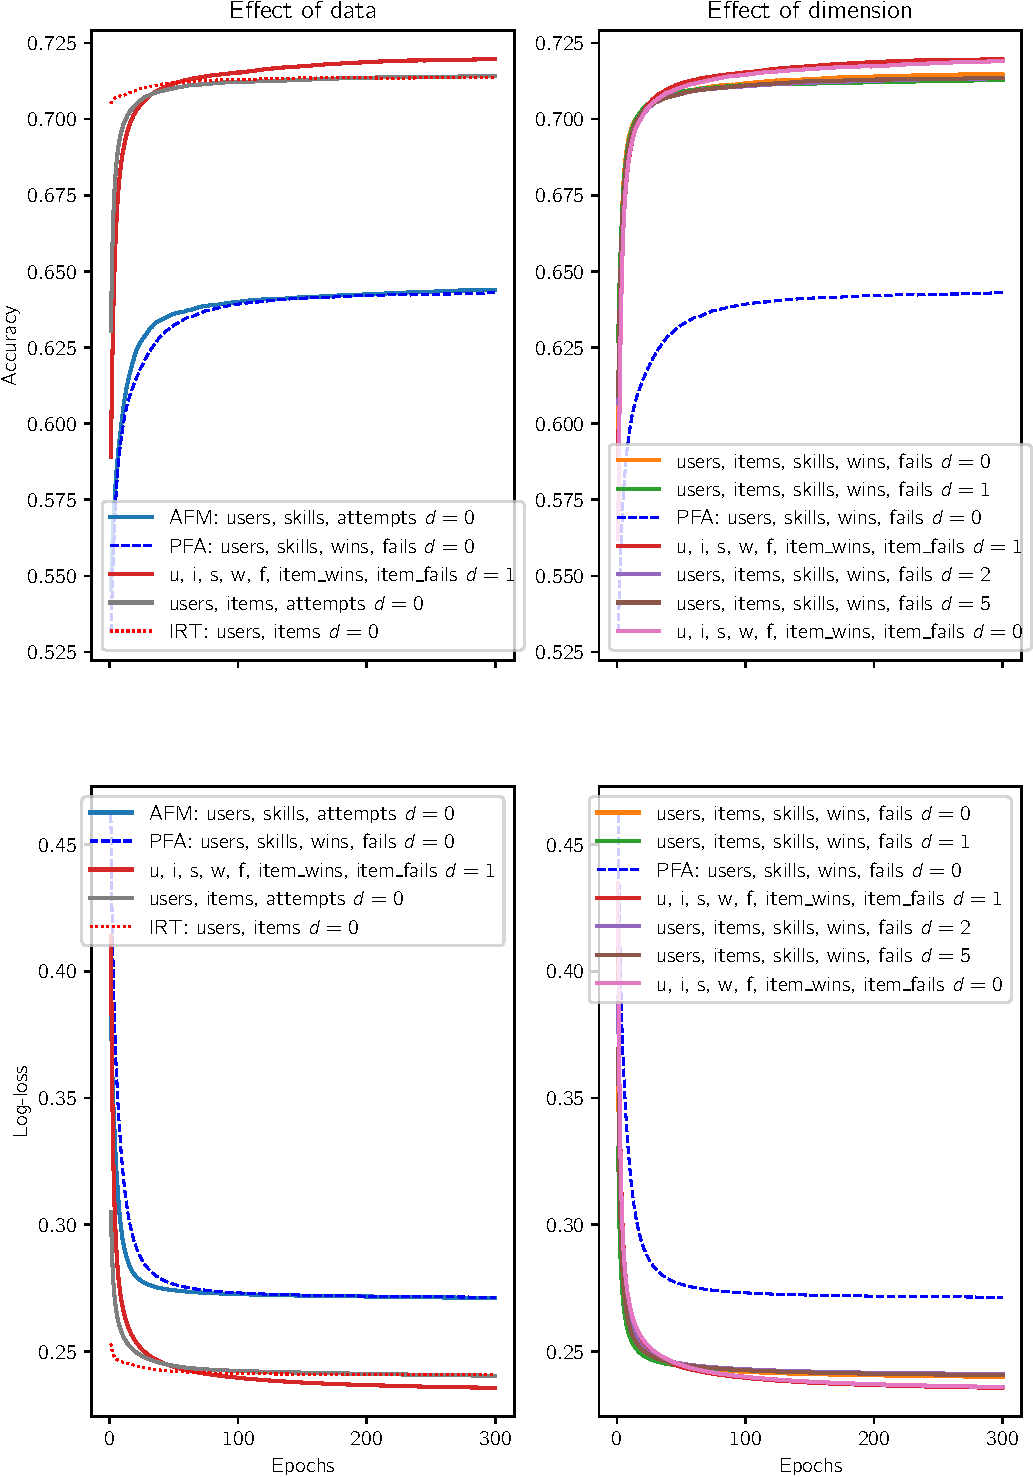
\includegraphics[width=0.50\linewidth]{figures/berkeley0-poster.pdf}\vspace{1cm}\\
    \begin{tabular}{lllllllll}
\toprule
AUC &     PFA &     AFM &              IRT &          MIRTb10 &        KTM(uia0) &        KTM(uis0) &       KTM(uis10) &    KTM(uiswfWF1) \\
\midrule
assistments &  0.7361 &  0.7366 &           0.7748 &               -- &  \textbf{0.7932} &               -- &               -- &           0.7882 \\
berkeley    &     0.7 &  0.7005 &           0.7856 &               -- &           0.7873 &               -- &               -- &  \textbf{0.7971} \\
castor6e    &      -- &      -- &  \textbf{0.8239} &           0.8235 &               -- &  \textbf{0.8240} &  \textbf{0.8239} &               -- \\
fraction    &      -- &      -- &           0.9124 &           0.9126 &               -- &           0.9125 &  \textbf{0.9146} &               -- \\
timss2003   &      -- &      -- &           0.7979 &           0.7979 &               -- &  \textbf{0.7999} &           0.7981 &               -- \\
\bottomrule
\end{tabular}

}


\column{.45}
\block{Better models found}{
    \begin{itemize}
    \item It is better to learn a item bias
    \item Bigger dimensions do not help much, sometimes harm
    \item IRT is simple yet competitive
    \end{itemize}
    \begin{tabular}{ccccc}
\toprule
                                  model &  dim &             ACC &             AUC &             NLL \\
\midrule
 users, items, skills, wins, fails, item\_wins, item\_fails &  1 &  \textbf{0.720} &  \textbf{0.797} &  \textbf{0.236} \\
 users, items, skills, wins, fails, item\_wins, item\_fails &  0 &  \textbf{0.719} &  \textbf{0.797} &  \textbf{0.236} \\
 users, items, skills, wins, fails &  0 &  0.715 &  0.788 &  0.24 \\
 users, items, attempts &  0 &  0.714 &  0.787 &  0.24 \\
 users, items, skills, wins, fails &  5 &  0.714 &  0.787 &  0.241 \\
 IRT: users, items &  0 &  0.714 &  0.786 &  0.241 \\
 users, items, skills, wins, fails &  2 &  0.713 &  0.786 &  0.241 \\
 users, items, skills, wins, fails &  1 &  0.713 &  0.786 &  0.241 \\
 MIRTb: users, items &  1 &  0.71 &  0.781 &  0.243 \\
 AFM: users, skills, attempts &  0 &  0.644 &  0.701 &  0.271 \\
 PFA: users, skills, wins, fails &  0 &  0.643 &  0.7 &  0.271 \\
\bottomrule
\end{tabular}

}
\block{Optimizing Human Learning}{
    We are organizing a workshop in Montréal on \textbf{June 12}:\\
    CFP open on \url{humanlearn.io}
}
\block{References}{
    \printbibliography[heading=none]
}
\end{columns}

\end{document}

\endinput
